\section{Analyse de la sévérité de façon univariée}\label{Section_Severite}
	Comme il est expliqué dans \cite{Parodi2015_Pricing_in_GenIns}(p.225) et dans \cite{TheorieDuRisque2018_MarceauEtCossette}(p.79), les lois de sévérités qui sont généralement à privilégier en contexte d'assurance sont des lois continues avec un support sur les réels positifs et possédants une asymétrie positive. De plus, comme Parodi l'explique dans son ouvrage, les lois les plus simples (moins de paramètres) sont souvent les meilleures candidates pour la modélisation. En effet, selon la théorie de l'apprentissage statistique, un modèle plus complexe que nécessaire offre un faible pouvoir de prédiction. Par ailleurs, des tests de comparaison tels que le critère d'information d'Akaike (AIC) ou le critère d'information bayésien de Schwartz (BIC) pénalisent le nombre de paramètres. Pour cette raison il faut vérifier l'adéquation des modèles univariés avant de regarder les modèles avec raccordement.\\
	
	Pour débuter l'analyse univariée, il serait intéressant de regarder plus en détail le comportement de la fonction d'excès moyen expliqué dans l'illustration \ref{Graph_MeanExcess} pour identifié les lois à utiliser. Ainsi, dans l'illustration \ref{Graph_MeanExcess}, on voit les principales lois utilisées pour ce travail.
	
	\begin{figure}[H]
		\begin{center}
		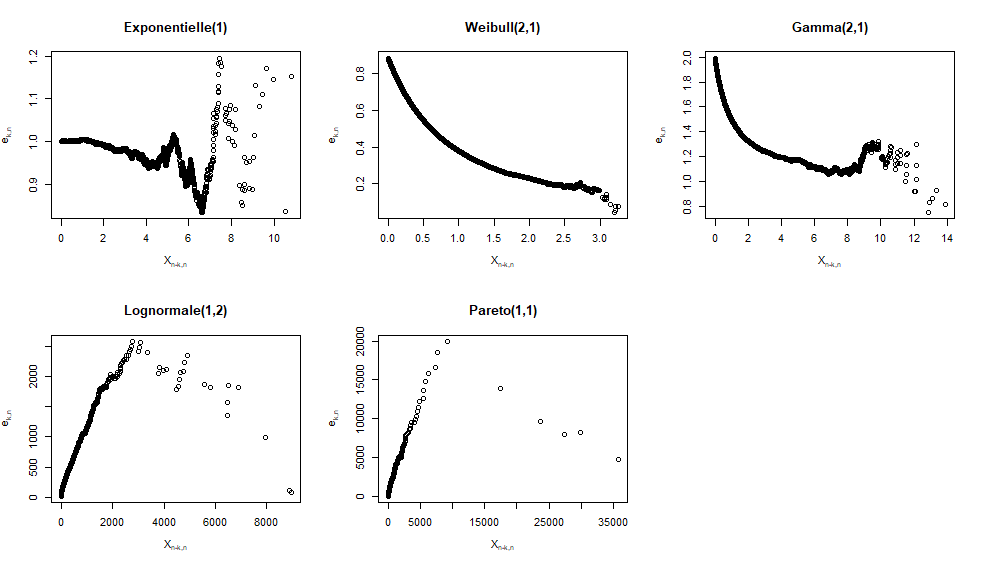
\includegraphics[scale=0.7]{Graphiques/Graph_MeanExcess} 
		\renewcommand{\figurename}{Illustration}
		\caption{Simulation du comportements de la fonction d'excès moyen selon le type de loi.} \label{Graph_MeanExcess}
	\end{center}
	\end{figure}

	Le premier constat de cette analyse graphique est qu'il ne faut pas nécessairement se fier sur les valeurs extrêmes de cette fonction pour définir des raccordement. En effet, ces graphiques ont été générés par simulation avec le code informatique \ref{Code_MeanExcess_Graphs}. Bien qu'il s'agisse de simulations de lois paramétriques, des valeurs aberrantes apparaissent dans la queue de la fonction d'excès moyen. \\
	
	\begin{Code}\label{Code_MeanExcess_Graphs}
		\begin{verbatim}
		
		set.seed(20181128)
		m <- 10^5
		par(mfrow=c(2,3))  
		MeanExcess(rexp(m),main = "Exponentielle(1)")
		MeanExcess(rweibull(m,2,1),main = "Weibull(2,1)")
		MeanExcess(rgamma(m,2,1),main = "Gamma(2,1)") 
		MeanExcess(rlnorm(m,1,2),main = "Lognormale(1,2)")
		MeanExcess(rpareto(m,1,1),main = "Pareto(1,1)")
		\end{verbatim}
	\end{Code}

	Le meilleur exemple de ce constat se produit avec la loi exponentielle. Comme celle-ci possède la propriété sans mémoire, la fonction d'excès moyen devrait être une constante. C'est à dire qu'on devrait observer une ligne droite. Cependant, comme on le voit dans l'illustration \ref{Graph_MeanExcess}, à partir du moment où on aperçoit des soubresauts dans la courbe, la fonction d'excès moyen ne semble plus être un bon indicateur de la loi.\\
	
	La raison qui explique ce phénomène est que l'estimateur empirique de la fonction d'excédent est une moyenne. Lorsque le nombre d'observations constituant cette moyenne diminue, la variabilité de l'estimateur augmente significativement. \\
	
	Pour aller plus en profondeur dans l'analyse graphique avec la fonction d'excès moyen, il faudrait simuler les mêmes graphiques avec différents ancrages (\textit{seeds}) pour observer la volatilité des courbes résultantes. Puis il faudrait refaire cette procédure avec différents paramètres. Cependant, considérant le laps de temps imparti pour ce travail, cette tâche devra être déléguée à d'autres.\\
	
	Malgré tout, les hypothèses énoncées dans l'analyse préliminaire demeurent pertinentes et différents modèles de raccordements son étudiés. Ces derniers sont abordés en détail dans la section \ref{Section_Splicing}.\\
	
	Maintenant, en regard de cette information, la première étape est de venir confirmer (ou infirmer) les hypothèses soulevées lors de l'analyse préliminaire du point de vue des montants de sinistre. \\
	
	De cette façon, pour la base de données \texttt{norwegianfire}, les lois les plus plausibles sont la loi de Pareto et la loi lognormale. Finalement, il serait intéressant de tester si un raccordement de lois peut offrir une meilleure adéquation qu'un modèle univariée.\\
	
	En ce qui concerne la base de données \texttt{secura}, on fait l'hypothèse qu'une loi de la famille exponentielle peut bien modéliser le corps de la distribution. Puis, un raccordement avec une loi de Pareto permet de modéliser les valeurs extrêmes. Parmi les lois de la famille exponentielle, mentionnons la loi exponentielle comme telle, la loi Weibull, la loi gamma et les mélanges d'Erlang. Concernant cette dernière classe, il existe un cas particulier qui est intéressant à expérimenter par ses propriétés analytiques, soit la loi coxienne (voir \cite{LossModels_FurtherTopics_Klugman2013}(p.3-10)). Cette dernière permet de trouver une forme analytique à des expressions complexes telles que le calcul de la $TVaR$ avec des données agrégées.
	Plus précisément, puisqu'il est avisé de limiter le nombre de paramètres afin de conserver le pouvoir prédictif du modèle, on utilise la loi coxienne d'ordre deux puisque celle-ci n'a que trois paramètres.\\
	
	Finalement, pour la base de données \texttt{danish}, on suppose dans la section \ref{Section_AnalysePreliminaire} qu'une loi de Pareto est le modèle le plus adéquat pour effectuer la modélisation de la sévérité des sinistres. \\
	
	\subsection{Paramétrisation des lois de sévérité}
	Peu importe que le modèle soit avec ou sans raccordement, l'étape de la paramétrisation est cruciale pour obtenir un modèle prédictif précis. Pour cette raison, comme dans le cas de l'analyse de la fréquence, la méthode du maximum de vraisemblance est utilisée.\\
	
	Par ailleurs, comme les données étudiées dans le présent travail comporte des troncatures, cela signifie que les fonctions de vraisemblance sont produites à l'aide des fonctions de densité conditionnelles. Dans la présente section, on voit comment les paramètres ont été estimés pour chacune des lois à l'étude.
		\subsubsection{Exponentielle}
			Soit $f_{X|X>d}(x)= \lambda e^{-\lambda(x-d)} \;, x>d\;,\lambda>0$, la fonction de densité conditionnelle d'une loi exponentielle. Alors la fonction du maximum de vraisemblance pour trouver le paramètre $\lambda$ est
			\begin{align*}
				\mathcal{L}(x,\lambda)
				&=\prod_{i=1}^{n} \lambda e^{-\lambda(x_i-d)}\\
				&=\lambda^n \exp\left\lbrace \sum_{i=1}^{n}-\lambda(x_i-d) \right\rbrace.
			\end{align*}
			La fonction de log-vraisemblance négative devient
			\begin{align*}
				-l(x,\lambda)
				&= -n \ln \lambda + n\lambda(\bar{x}-d).		
			\end{align*}
			En dérivant par rapport à $\lambda$ et en égalisant le résultat à zéro, 
			$$	\frac{\textrm{d}}{\textrm{d}\lambda} l(x,\lambda) = -\frac{n}{\lambda}+ n(\bar{x}-d) = 0,$$ \\
			on déduit	$$ \hat{\lambda} = \frac{1}{\bar{x}-d},$$
			qui correspond au meilleur estimateur de $\lambda$ selon la méthode du maximum de vraisemblance.
		\subsubsection{Weibull}
			Pour la loi Weibull, l'expression de la fonction de densité conditionnelle est 
			$$ f_{X|X>d}(x)=\beta\tau(\beta x)^{\tau-1} e^{(\beta d)^\tau - (\beta x)^\tau}\;,x>d\;,\tau>0\;, \beta>0.$$
			
			Dans ce cas-ci, les paramètres sont trouvés par optimisation numérique grâce au code informatique \ref{Code_Mle_Weibull}
			\begin{Code}\label{Code_Mle_Weibull}
				\begin{verbatim}
				
				neg_log_vrais <- function(para){
				-sum(log(dweibull(LOSS,para[1],para[2])/(1-pweibull(d,para[1],para[2]))))
				}
				
				mle_Weibull <- constrOptim(c(2, 10^6), neg_log_vrais, grad = NULL, 
				ui = diag(2), ci = c(0,0))
				\end{verbatim}
			\end{Code}
			
		\subsubsection{Gamma}
		Dans le cas de la loi Gamma, la fonction de densité conditionnelle est donné par 
		$$f_{X|X>d}(x)= \frac{\lambda^\alpha x^{\alpha-1} e^{-\lambda(x)}/\Gamma(\alpha)}{\bar{H}(d;\alpha,\lambda)} \;, x>d\;,\alpha>0 \;,\lambda>0 ,$$ 
		où $\bar{H}$ correspond à la fonction de survie d'une loi gamma.\\
		
		Le code informatique \ref{Code_Mle_Gamma} présente la façon de trouver les paramètres selon la méthode du maximum de vraisemblance.
		\begin{Code}\label{Code_Mle_Gamma}
		\begin{verbatim}
		
		neg_log_vrais <- function(para){
		-sum(log(dgamma(LOSS,para[1],para[2])/(1-pgamma(d,para[1],para[2]))))
		}
		
		mle_gamma <- constrOptim(c(10, 1/5000), neg_log_vrais, grad = NULL, 
		ui = diag(2), ci = c(0,0),outer.eps = .Machine$double.eps)
		\end{verbatim}
		\end{Code}

		Comme pour l'estimation des paramètres d'un processus de Poisson non homogène, la méthode des moments est tout à fait adéquate pour estimer les paramètres initiaux de la loi.\\
		
		Selon l'importance de la troncature, il peut être possible d'utiliser cette méthode sans considérer le conditionnement. Advenant que la troncature soit trop importante, en revanche, cette méthode devient rapidement très complexe, voir même d'aucune utilité. À ce moment, il faut y aller de façon analytique (selon le contexte) et faire de l'essai-erreur. \\
		
		À noter que, dans le cas de la loi gamma, il est difficile d'estimer les paramètres, même avec la méthode algorithmique, lorsque la base de données possède une queue de distribution épaisse. Il faut donc tronquer ces données qui font diverger l'algorithme avant d'en estimer les paramètres.
		
		\subsubsection{Lognormale}
		Pour la loi lognormale, la fonction de densité conditionnelle est 
		$$f_{X|X>d}(x) = \frac{\exp\left\lbrace -\frac{1}{2}(\frac{\ln x-\mu}{\sigma})^2\right\rbrace }{x\sqrt{2\pi}\sigma * (1-\Phi(\frac{\ln x - \mu}{\sigma}))}\;, x>d \;, -\infty < \mu < \infty \;, \sigma^2 >0,$$
		où $\Phi$ est la fonction de répartition d'une loi normale centrée et réduite.\\
		
		En termes général, il est relativement aisé d'estimer algébriquement les paramètres de la loi lognormale. Cependant étant donné le conditionnement, il faudra utiliser une méthode d'optimisation numérique. Ainsi, le code informatique \ref{Code_Mle_LogNormale} permet d'y parvenir.
		\begin{Code}\label{Code_Mle_LogNormale}
			\begin{verbatim}
			
			neg_log_vrais <- function(para){
			-sum(log(dlnorm(LOSS,para[1],para[2])/(1-plnorm(d,para[1],para[2]))))
			}
			
			mle_lnorm <- constrOptim(c(1, 1), neg_log_vrais, grad = NULL, 
			ui = c(0,1), ci = 0,outer.eps = .Machine$double.eps)
			\end{verbatim}		
		\end{Code}

		
		\subsubsection{Pareto}
		Dans le contexte de la loi de Pareto, la fonction de densité conditionnelle est
		$$f_{X|X>d}(x) = \frac{\alpha(\lambda + d)^\alpha}{(\lambda + x)^{\alpha+1}}\;, x>d\;,\lambda>0\;,\alpha>0.$$
		Le code informatique \ref{Code_Mle_Pareto} permet d'estimer les paramètres de la loi de Pareto par optimisation numérique.
		\begin{Code}\label{Code_Mle_Pareto}
		\begin{verbatim}
		
		neg_log_vrais <- function(para){
		-sum(log(dpareto(LOSS,para[1],para[2])/(1-ppareto(d,para[1],para[2]))))
		}
		
		mle_pareto <- constrOptim(c(3, 6), neg_log_vrais, grad = NULL, 
		ui = diag(2), ci = c(0, 0),outer.eps = .Machine$double.eps)
		\end{verbatim}
		\end{Code}
	
		\subsubsection{Coxienne-2}
		La loi coxienne-2 admet la fonction de densité suivante :
		$$f_{X|X>d}(x) = \frac{p\beta_1 e^{-\beta_1 x} + (1-p) \beta_1 \beta_2 \left( \frac{ e^{-\beta_1 x}}{\beta_2 - \beta_1} + \frac{ e^{-\beta_2 x}}{\beta_1 - \beta_2}\right)}
		{p e^{-\beta_1 d} + (1-p)  \left( \frac{\beta_2}{\beta_2 - \beta_1}e^{-\beta_1 d} + \frac{\beta_1}{\beta_1 - \beta_2}e^{-\beta_2 d}\right)}\;, x>d\;, \beta_1 \neq \beta_2. $$
		
		Afin de trouver les estimateurs des paramètres par optimisation numérique, il suffit utiliser le code informatique \ref{Code_Mle_Cox2}.
		\begin{Code}\label{Code_Mle_Cox2}
		\begin{verbatim}
		
		neg_log_vrais <- function(para){
		-sum(log(fx1(LOSS,para[1],para[2],para[3])/(1-Fx1(d,para[1],para[2],para[3]))))
		}
	
		mle_Coxian2_est <- constrOptim(c(1/1000, 1/2000, 0.5), neg_log_vrais, grad = NULL, 
		ui = diag(3), ci = c(0,0,0))
		\end{verbatim}
		\end{Code}
		Pour de plus amples informations sur la loi coxienne-2, on peut consulter l'annexe se trouvant à la page \pageref{Annexe_Cox2} ou lire \cite{LossModels_FurtherTopics_Klugman2013} aux pages 3 à 10.\\
		
		Une fois que les paramétrisation des lois étudiées est faite, il s'agit de regarder quelles lois s'harmonisent le mieux avec les quantiles empiriques à l'aide de graphiques de quantiles à quantiles(\textit{QQplots}). Puis, si une ambiguïté est soulevée, des tests d'adéquation statistique sont utilisés pour départager la loi à utiliser. Les tests d'adéquation et le sélection de modèle est abordé plus en détail dans la section \ref{Sect_Adequation}.
		
		